\usepackage{graphicx}
\newpage
\thispagestyle{fancy}
\vspace{\fill}

\subsection{Vista geral dos ajustes das impressoras}
\begin{figure}
    \centering
    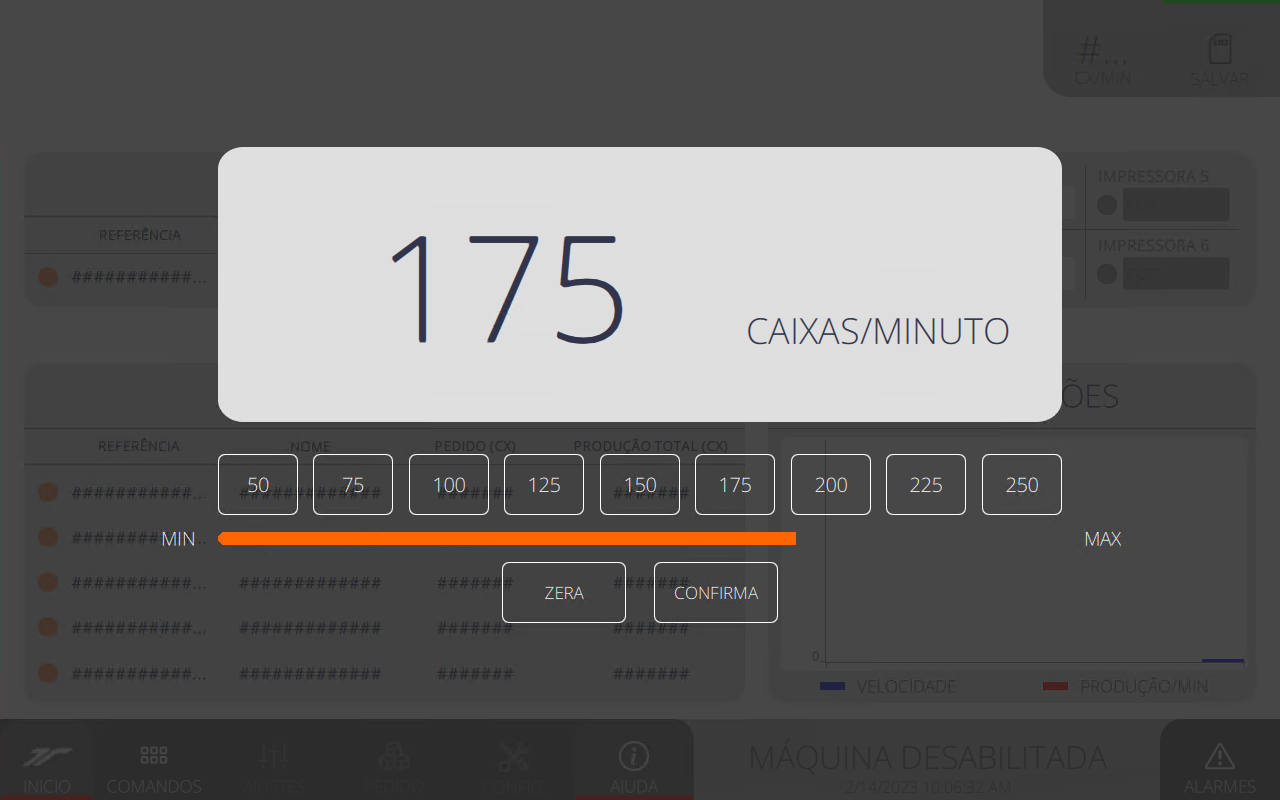
\includegraphics[width=480,height=300]{imagesICV/04-printters/01-printters/settings/1}
    \caption{Vista geral dos ajustes das impressoras}
\end{figure}
\newpage
\thispagestyle{fancy}
\vspace{\fill}

\subsection{Aproximação do anilox bloqueada}
\begin{figure}
    \centering
    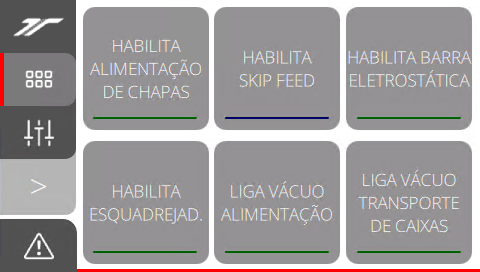
\includegraphics[width=576,height=360]{imagesICV/04-printters/01-printters/settings/2}
    \caption{Aproximação do anilox bloqueada}
\end{figure}
\newpage
\thispagestyle{fancy}
\vspace{\fill}

\subsection{Registro atual}
\begin{figure}
    \centering
    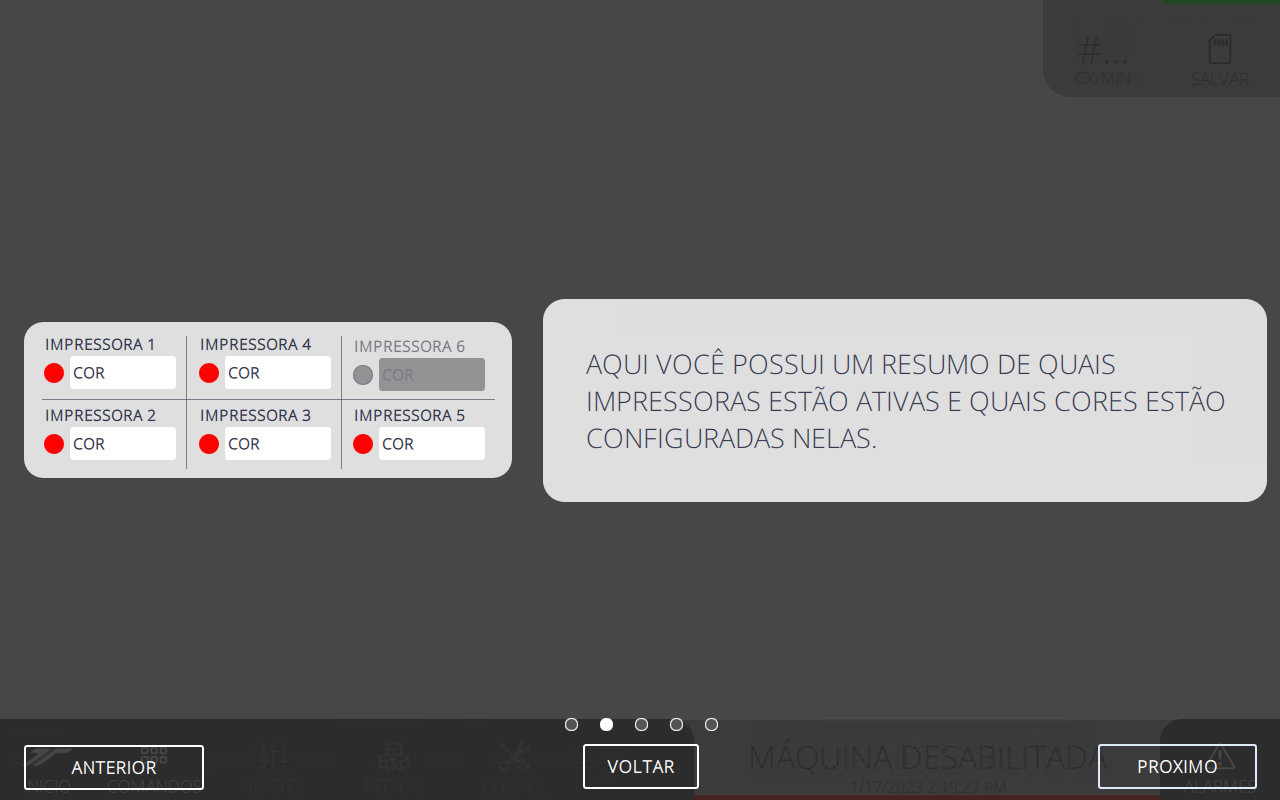
\includegraphics[width=576,height=360]{imagesICV/04-printters/01-printters/settings/3}
    \caption{Registro atual}
\end{figure}
\newpage
\thispagestyle{fancy}
\vspace{\fill}

\subsection{Ajuste axial do Clichê}
\begin{figure}
    \centering
    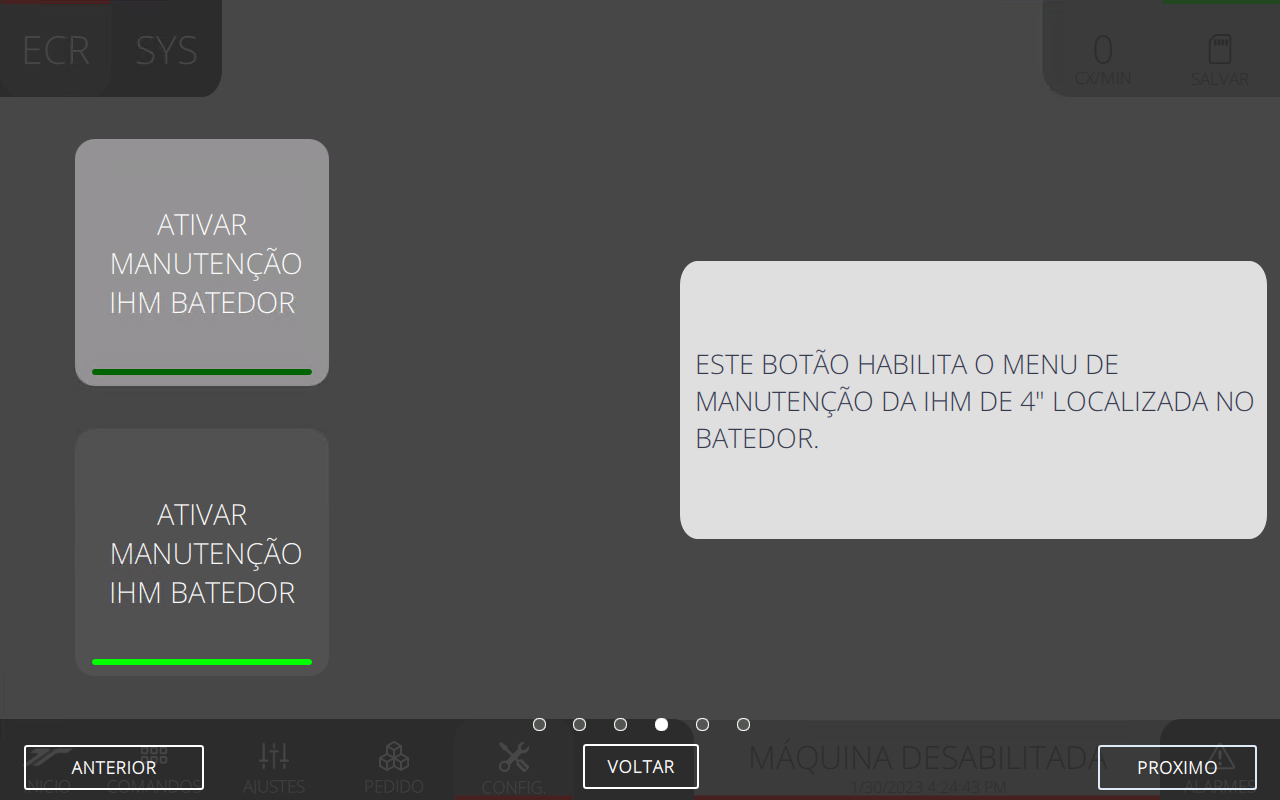
\includegraphics[width=576,height=360]{imagesICV/04-printters/01-printters/settings/4}
    \caption{Ajuste axial do Clichê}
\end{figure}
\newpage
\thispagestyle{fancy}
\vspace{\fill}

\subsection{Pressão caixa de vácuo}
\begin{figure}
    \centering
    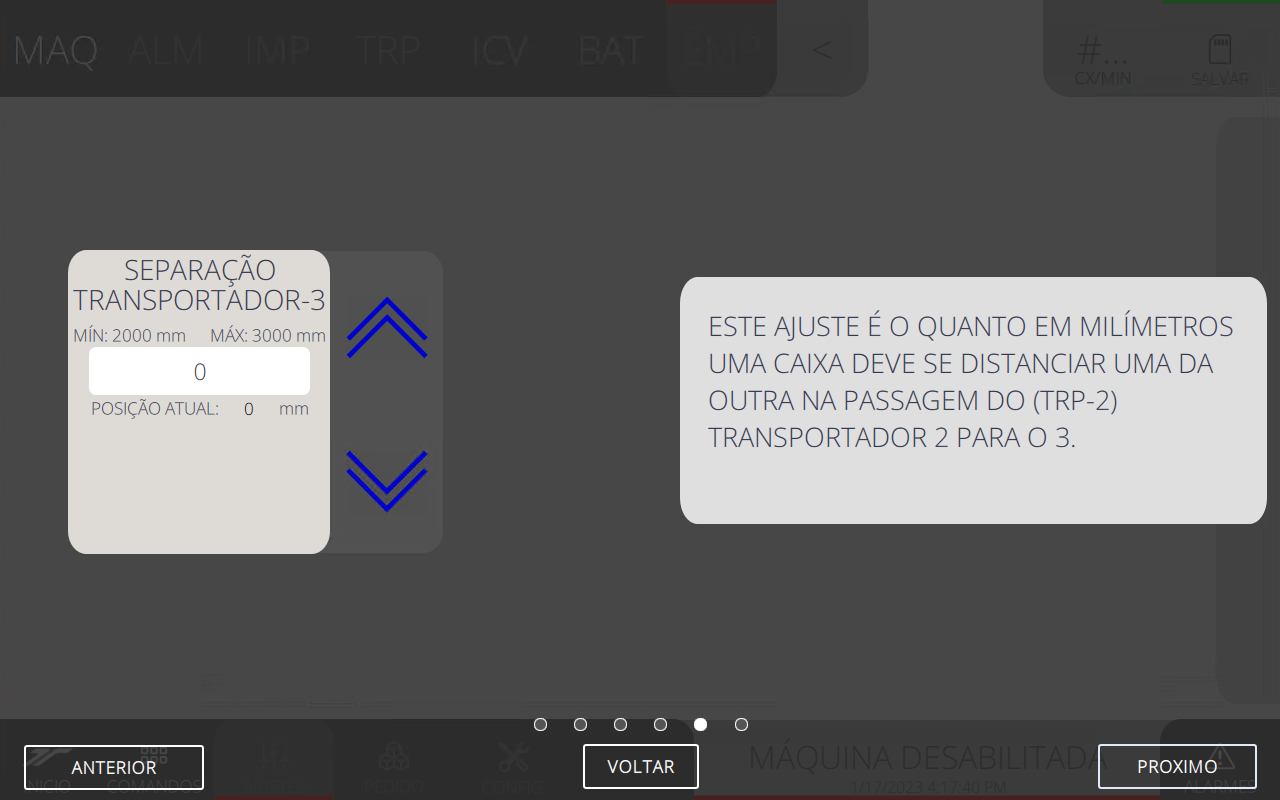
\includegraphics[width=576,height=360]{imagesICV/04-printters/01-printters/settings/5}
    \caption{Pressão caixa de vácuo}
\end{figure}
\newpage
\thispagestyle{fancy}
\vspace{\fill}

\subsection{Pressão anilox}
\begin{figure}
    \centering
    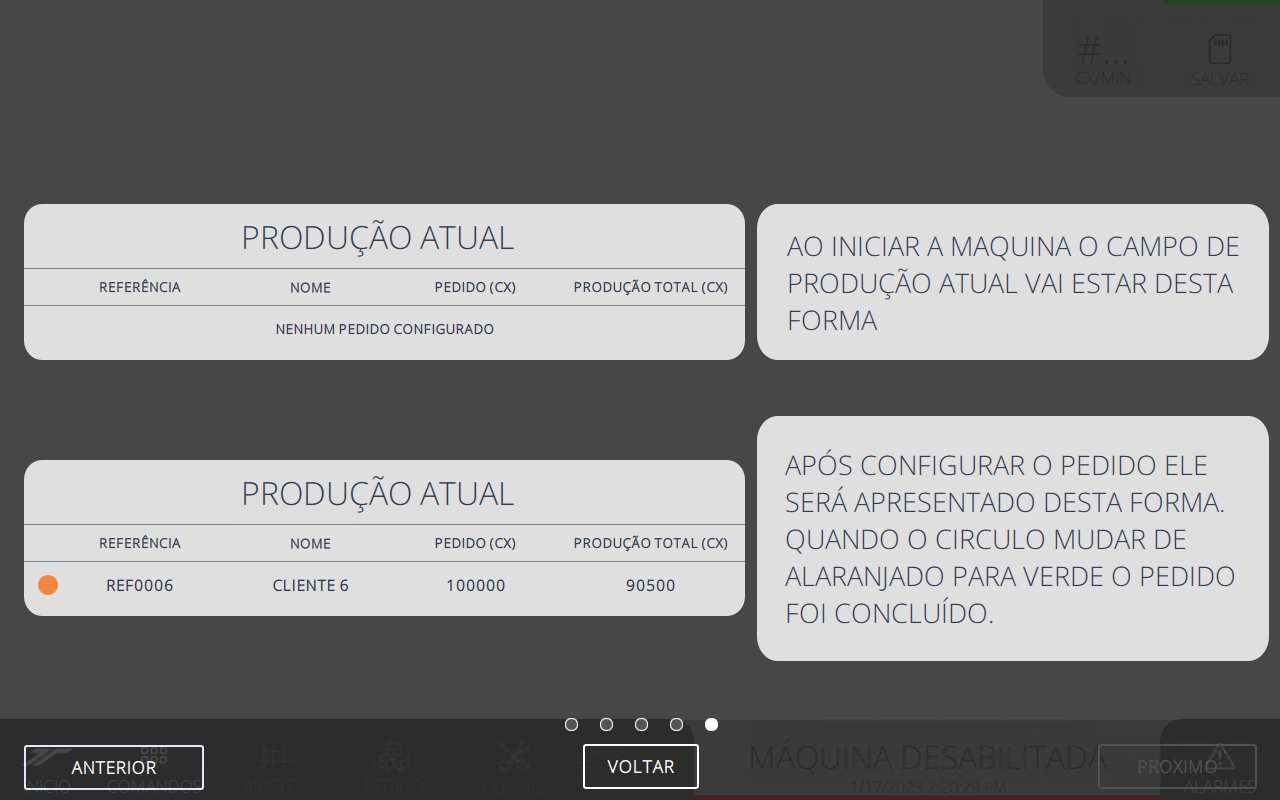
\includegraphics[width=576,height=360]{imagesICV/04-printters/01-printters/settings/6}
    \caption{Pressão anilox}
\end{figure}
\newpage
\thispagestyle{fancy}
\vspace{\fill}

\subsection{Intensidade do vácuo}
\begin{figure}
    \centering
    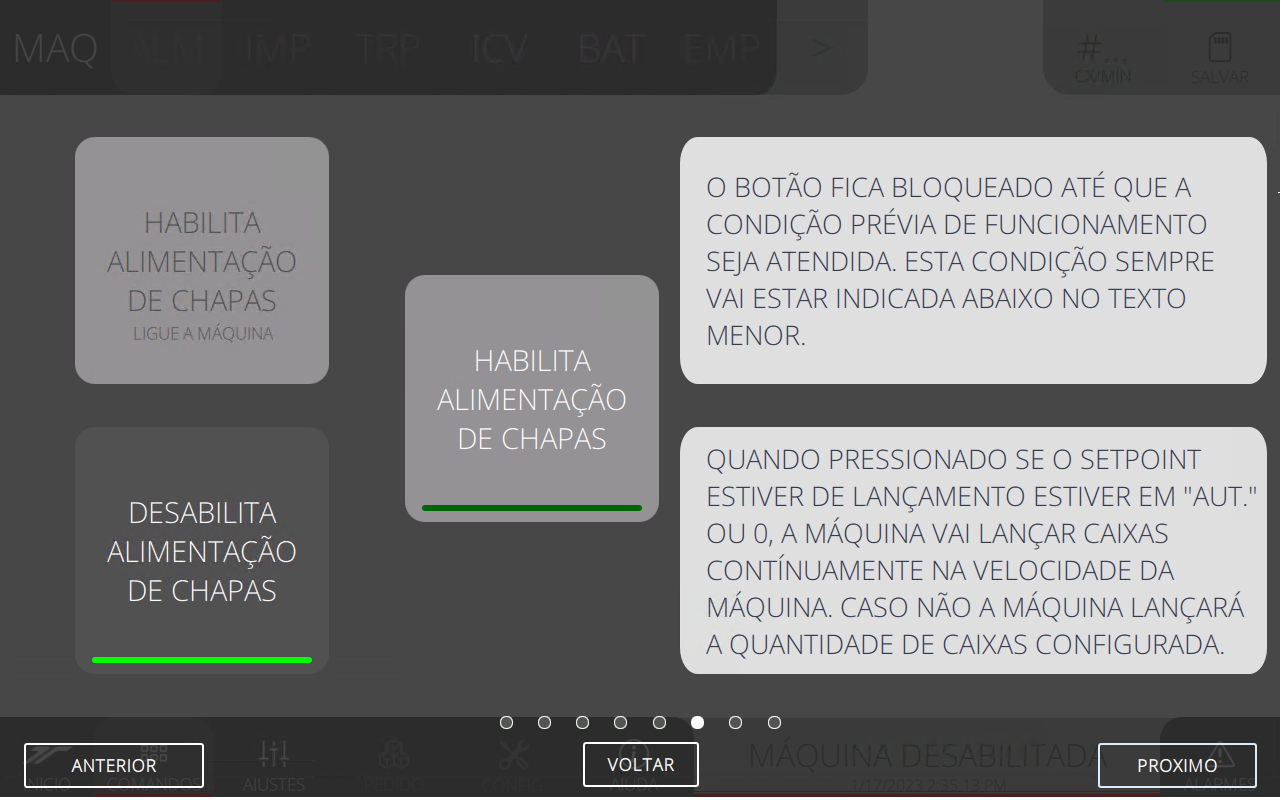
\includegraphics[width=576,height=360]{imagesICV/04-printters/01-printters/settings/7}
    \caption{Intensidade do vácuo}
\end{figure}
\newpage
\thispagestyle{fancy}
\vspace{\fill}

\subsection{Tempo ativo da lavagem de tinta}
\begin{figure}
    \centering
    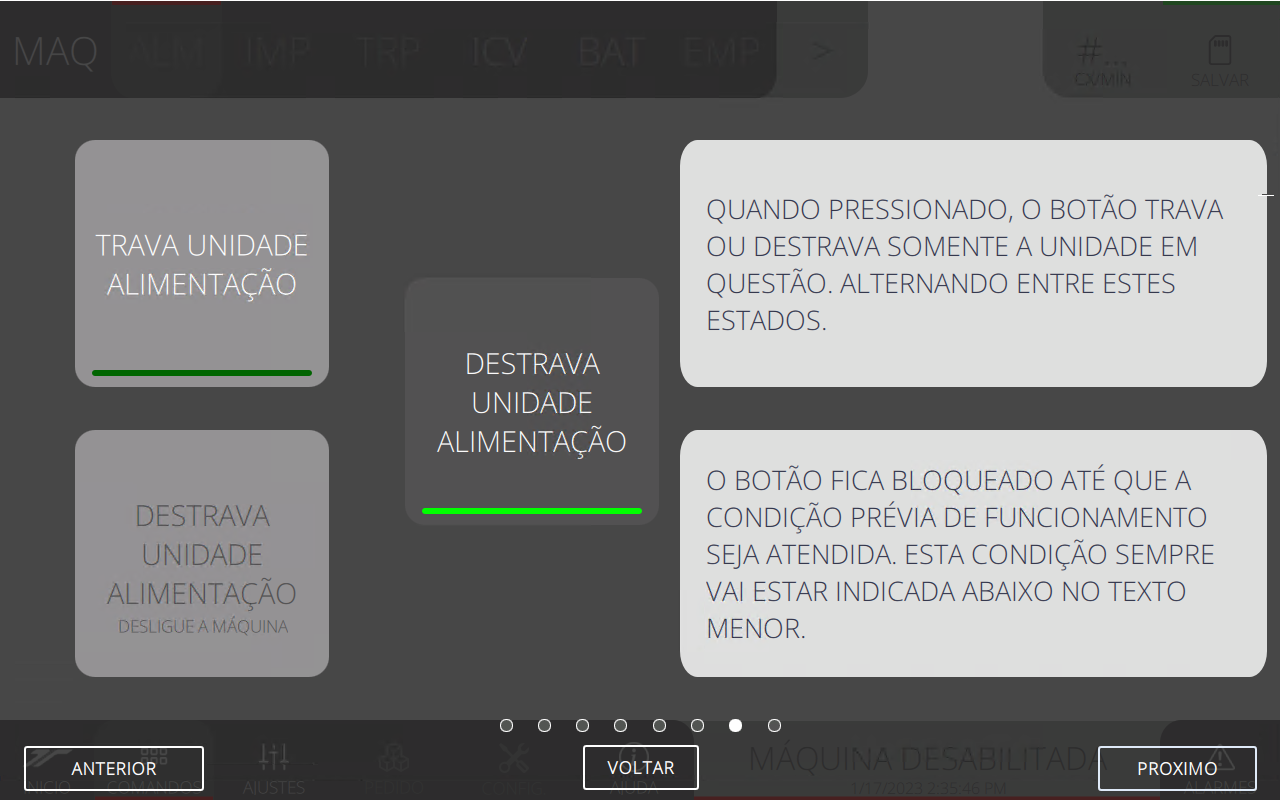
\includegraphics[width=576,height=360]{imagesICV/04-printters/01-printters/settings/8}
    \caption{Tempo ativo da lavagem de tinta}
\end{figure}
\newpage
\thispagestyle{fancy}
\vspace{\fill}

\subsection{Ajuste individual da unidade}
\begin{figure}
    \centering
    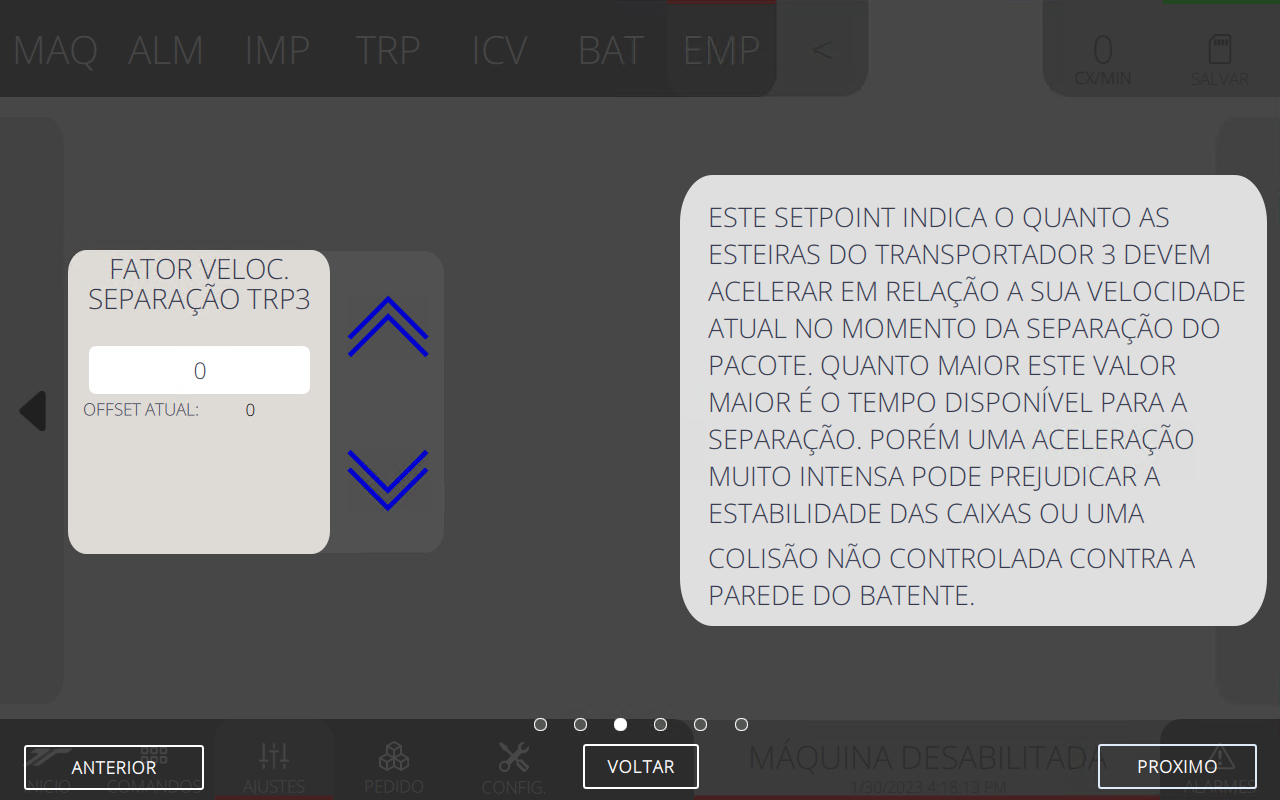
\includegraphics[width=576,height=360]{imagesICV/04-printters/01-printters/settings/9}
    \caption{Ajuste individual da unidade}
\end{figure}
\newpage
\thispagestyle{fancy}
\vspace{\fill}

\subsection{Axial porta clichê}
\begin{figure}
    \centering
    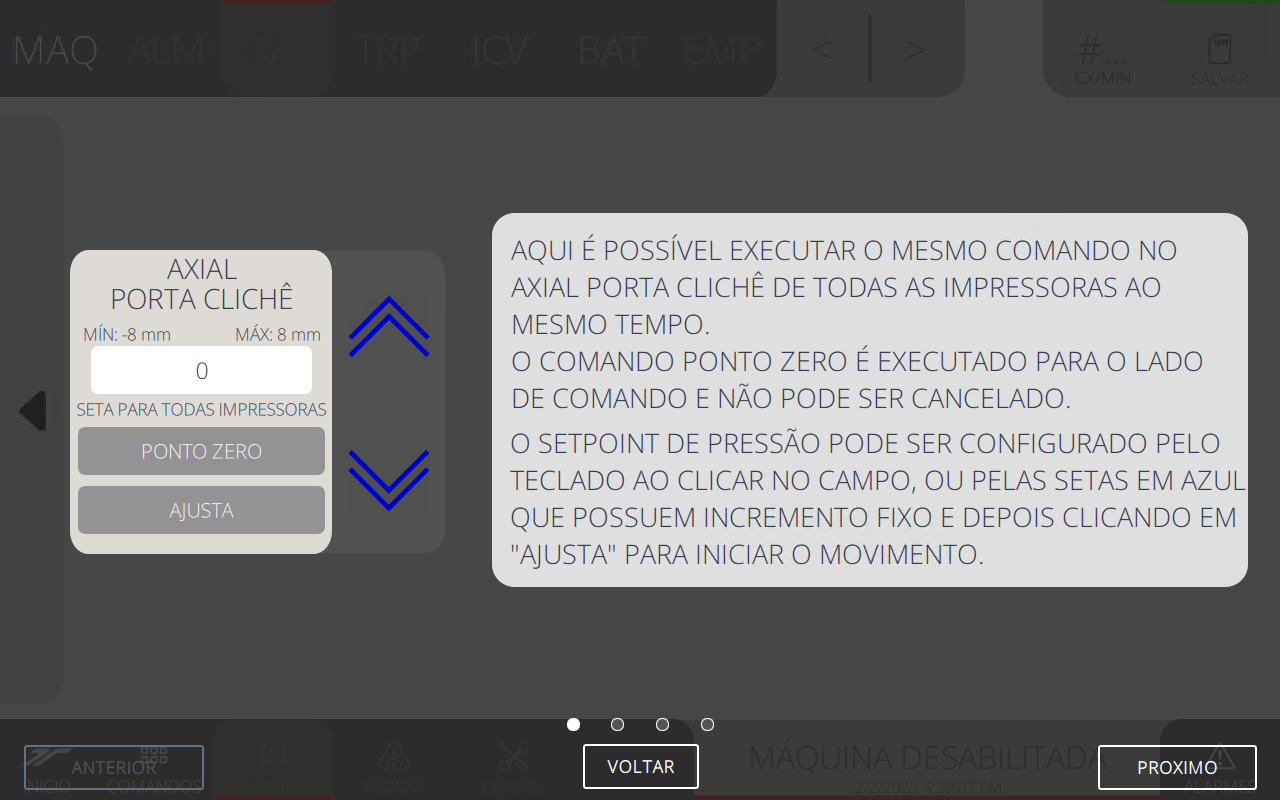
\includegraphics[width=576,height=360]{imagesICV/04-printters/01-printters/settings/10}
    \caption{Axial porta clichê}
\end{figure}
\newpage
\thispagestyle{fancy}
\vspace{\fill}

\subsection{Pressão caixa de vácuo}
\begin{figure}
    \centering
    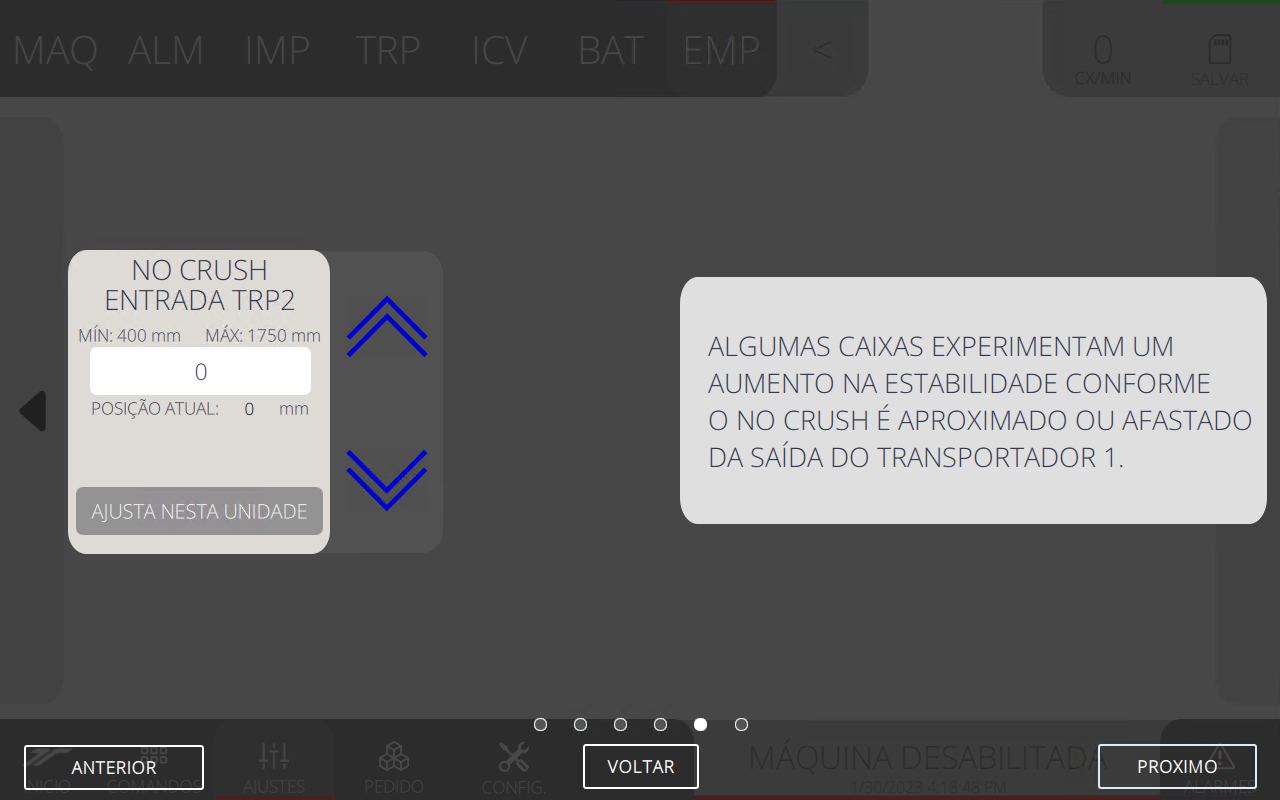
\includegraphics[width=576,height=360]{imagesICV/04-printters/01-printters/settings/11}
    \caption{Pressão caixa de vácuo}
\end{figure}
\newpage
\thispagestyle{fancy}
\vspace{\fill}

\subsection{Radial porta clichê}
\begin{figure}
    \centering
    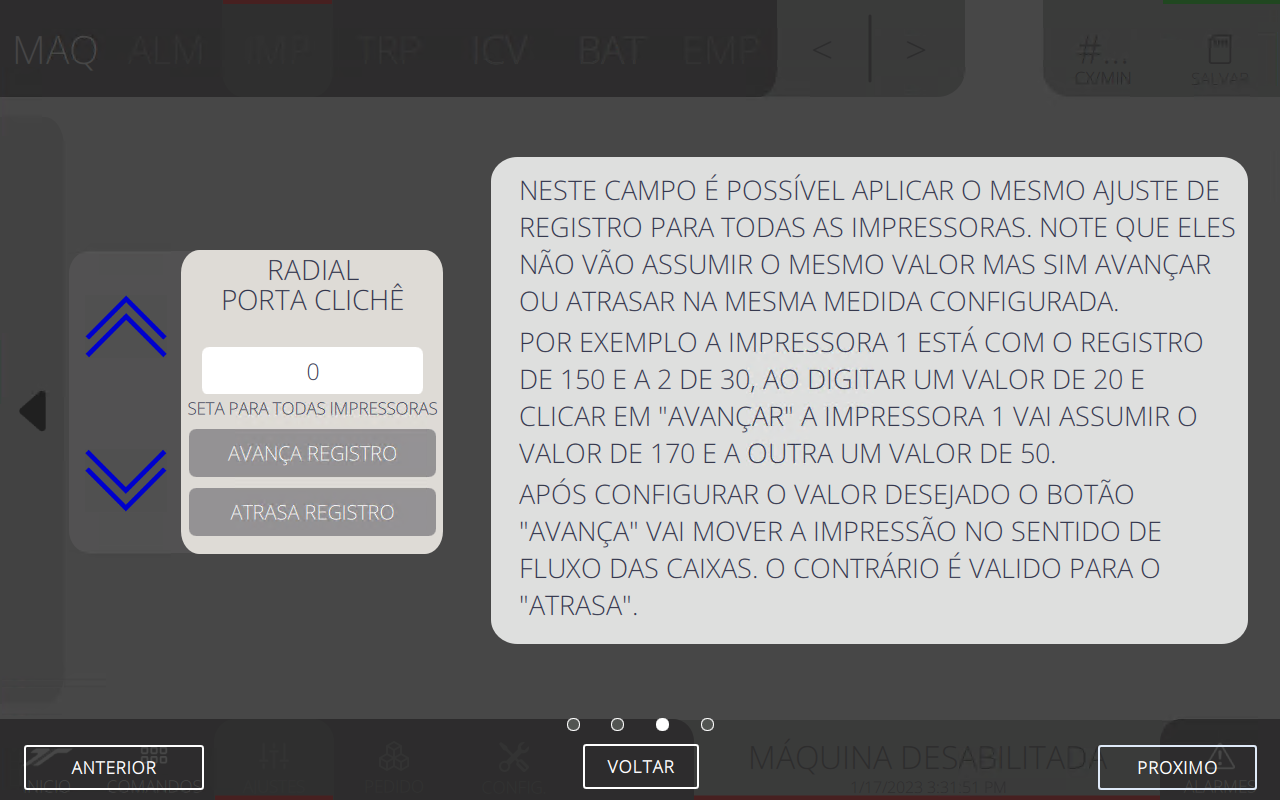
\includegraphics[width=576,height=360]{imagesICV/04-printters/01-printters/settings/12}
    \caption{Radial porta clichê}
\end{figure}
\newpage
\thispagestyle{fancy}
\vspace{\fill}

\subsection{Pressão rolo anilox}
\begin{figure}
    \centering
    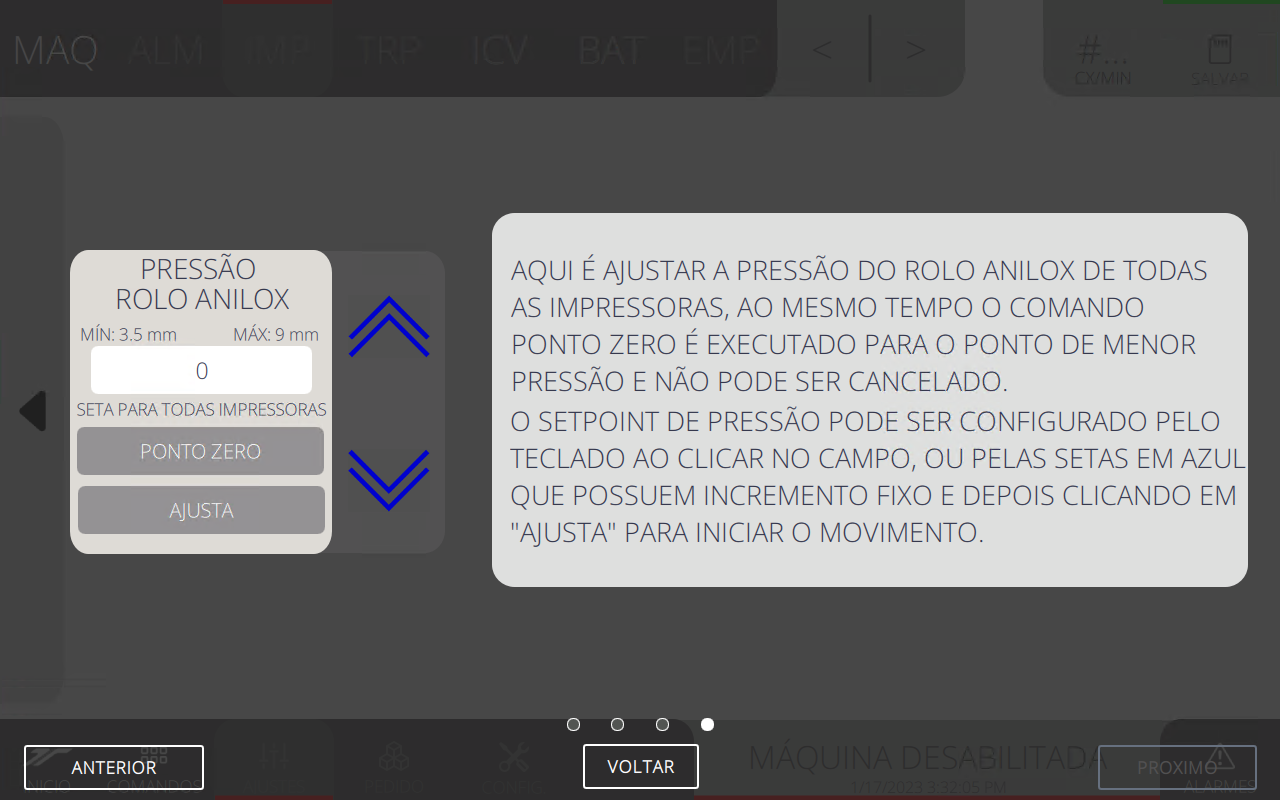
\includegraphics[width=576,height=360]{imagesICV/04-printters/01-printters/settings/13}
    \caption{}
\end{figure}